\documentclass{beamer}
\usepackage[utf8]{inputenc}

\usetheme{Madrid}
\usecolortheme{default}
\usepackage{amsmath,amssymb,amsfonts,amsthm}
\usepackage{txfonts}
\usepackage{multicol}
\usepackage{tkz-euclide}
\usepackage{listings}
\usepackage{adjustbox}
\usepackage{array}
\usepackage{tabularx}
\usepackage{gvv}
\usepackage{lmodern}
\usepackage{circuitikz}
\usepackage{tikz}
\usepackage{graphicx}
\usepackage{hyperref}

\setbeamertemplate{page number in head/foot}[totalframenumber]

\usepackage{tcolorbox}
\tcbuselibrary{minted,breakable,xparse,skins}



\definecolor{bg}{gray}{0.95}
\DeclareTCBListing{mintedbox}{O{}m!O{}}{%
  breakable=true,
  listing engine=minted,
  listing only,
  minted language=#2,
  minted style=default,
  minted options={%
    linenos,
    gobble=0,
    breaklines=true,
    breakafter=,,
    fontsize=\small,
    numbersep=8pt,
    #1},
  boxsep=0pt,
  left skip=0pt,
  right skip=0pt,
  left=25pt,
  right=0pt,
  top=3pt,
  bottom=3pt,
  arc=5pt,
  leftrule=0pt,
  rightrule=0pt,
  bottomrule=2pt,
  toprule=2pt,
  colback=bg,
  colframe=orange!70,
  enhanced,
  overlay={%
    \begin{tcbclipinterior}
    \fill[orange!20!white] (frame.south west) rectangle ([xshift=20pt]frame.north west);
    \end{tcbclipinterior}},
  #3,
}
\lstset{
    language=C,
    basicstyle=\ttfamily\small,
    keywordstyle=\color{blue},
    stringstyle=\color{orange},
    commentstyle=\color{green!60!black},
    numbers=left,
    numberstyle=\tiny\color{gray},
    breaklines=true,
    showstringspaces=false,
}
%------------------------------------------------------------
%This block of code defines the information to appear in the
%Title page
\title %optional
{5.8.2}
\date{September 27,2025}
%\subtitle{A short story}

\author % (optional)
{Aditya Appana - EE25BTECH11004}



\begin{document}


\frame{\titlepage}
\begin{frame}{Question}
10 students of Class X took part in a Mathematics quiz. If the number of girls is 4
more than the number of boys, find the number of boys and girls who took part in
the quiz.
\end{frame}



\begin{frame}[fragile]
    \frametitle{Solution}
Let the number of girls in the class be $g$, and the number of boys be $b$. Let the vector representing this data be 
\begin{align}
\vec{x} = \myvec{g\\b}    
\end{align}\\
Since the total number of students in the class is 10, $g+b=10$ which can be expressed as:
\begin{align}
\myvec{1\\1}^T\vec{x} = 10
\end{align}\\
Since there are 4 more girls than boys, $b+4=g$, which can be expressed as:
\begin{align}
\myvec{-1 \\ 1}^T\vec{x} = -4
\end{align}\\

\end{frame}


\begin{frame}[fragile]
    \frametitle{Solution}
    
Organising these two equations into the form $\vec{A}\vec{x} = \vec{b}$:
\begin{align}
\myvec{1&1 \\ -1&1} \vec{x} = \myvec{10\\-4}
\end{align}\\
Normalising $\vec{A}$: 
\begin{align}
\sqrt{2} \myvec{\frac{1}{\sqrt{2}} & \frac{1}{\sqrt{2}} \\  \frac{-1}{\sqrt{2}}& \frac{1}{\sqrt{2}}} \vec{x} = \myvec{10\\-4}
\end{align}
\end{frame}

\begin{frame}[fragile]
    \frametitle{Solution}
Let \myvec{\frac{1}{\sqrt{2}} & \frac{1}{\sqrt{2}} \\  \frac{-1}{\sqrt{2}}& \frac{1}{\sqrt{2}}} be $\vec{M}$. $\vec{M}$ is orthogonal, therefore $\vec{M^T}\vec{M} = \vec{I}$.\\
Multiplying by $\vec{M^T}$ on both the sides:
\begin{align}
\sqrt{2}\vec{x} = \myvec{\frac{1}{\sqrt{2}} & \frac{-1}{\sqrt{2}} \\  \frac{1}{\sqrt{2}}& \frac{1}{\sqrt{2}}} \myvec{10\\-4}\\
\vec{x} = \frac{1}{\sqrt{2}}\myvec{\frac{1}{\sqrt{2}} & \frac{-1}{\sqrt{2}} \\  \frac{1}{\sqrt{2}}& \frac{1}{\sqrt{2}}} \myvec{10\\-4}
\end{align}\\
Solving we get:\begin{align}
\vec{x} = \myvec{7\\3} \\
g = 7\\
b=3
\end{align}
\end{frame}





\begin{frame}[fragile]
    \frametitle{Python Code}

    \begin{lstlisting}
import numpy as np
import numpy.linalg 
import matplotlib.pyplot as plt

answer = numpy.linalg.solve([[1,1],[-1,1]], [10,-4])

answer[0] = round(answer[0],2)
answer[1] = round(answer[1],2)
print(answer)
\end{lstlisting} 
\end{frame}

\begin{frame}[fragile]
    \frametitle{Python Code}

    \begin{lstlisting}


fig = plt.figure(figsize =(6,6))
ax = fig.add_subplot(111)

X = np.linspace(-20,20,2)

Y1 = (10-X)
Y2 = (X-4)

ax.plot(X, Y1, label='Line 1')
ax.plot(X, Y2, label='Line 2')
ax.scatter(answer[0], answer[1], label=f'({answer[0]}, {answer[1]})')
ax.grid(True)
ax.legend()
plt.show()

    \end{lstlisting}
\end{frame}

\begin{frame}[fragile]
\frametitle{Plot}

\begin{figure}[H]
    \centering
    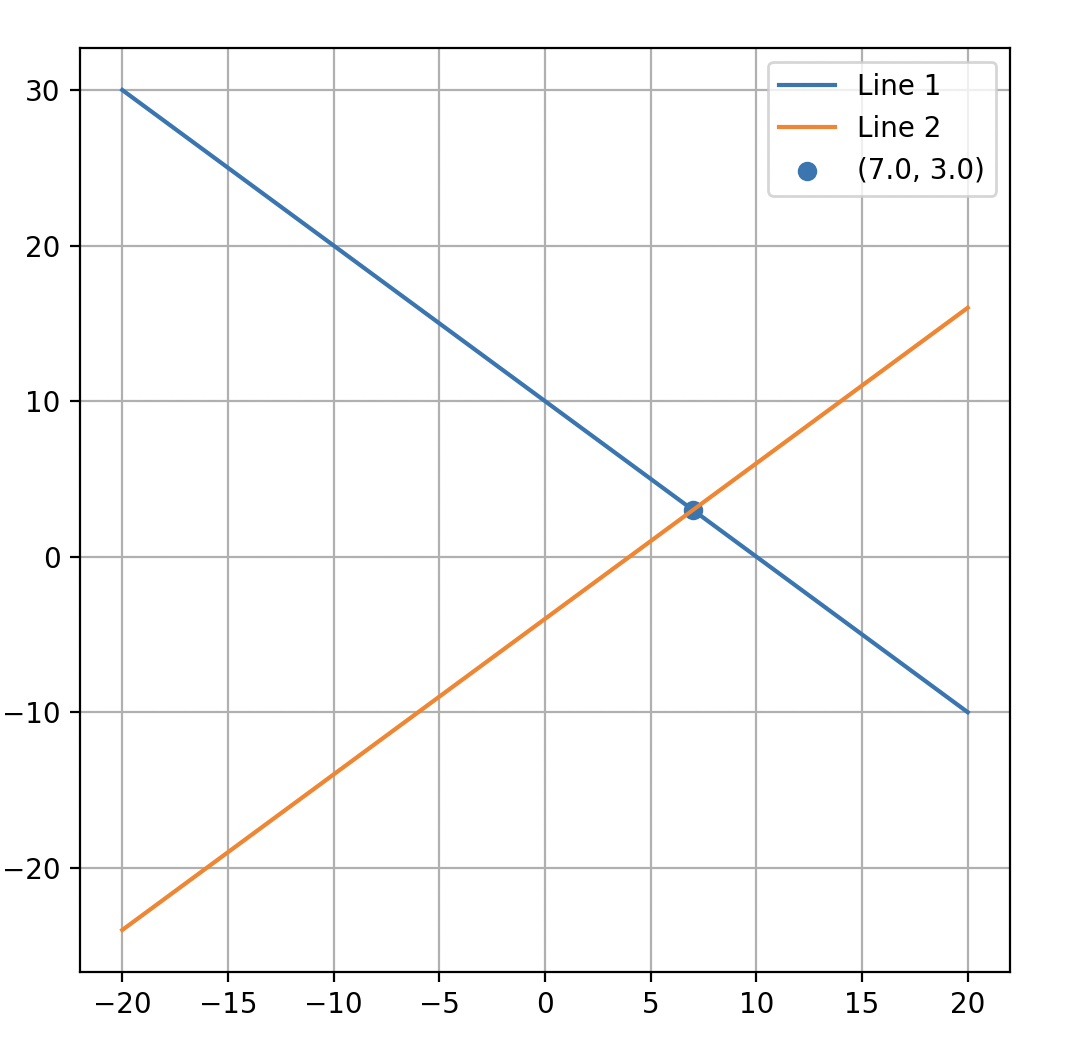
\includegraphics[width=0.6\columnwidth]{Figs/582.png}
    \caption{Plot}
    \label{fig:placeholder}
\end{figure}

\end{frame}
\end{document}